\chapter{Zapewnianie jakości i konserwacja systemu}
\label{Chapter7}

\section{Testy i weryfikacja jakości oprogramowania}
\label{Chapter71}

\subsection{Wstęp}
\label{Chapter711}

Testy i weryfikacja jakości oprogramowania realizowana była na trzech poziomach: testów jednostkowych (dla logiki) oraz automatycznych i manualnych testów akceptacyjnych. Te ostatnie realizowane były nie tylko w zgodzie z dokumentem \textit{MAT}\cite{Redmine:ProjDocs}, ale też intuicyjnie, poprzez zwykłe korzystanie z systemu.

\subsection{Testy jednostkowe}
\label{Chapter712}

Testy jednostkowe zostały wykonane jako pierwsze i traktowane były z wysokim priorytetem. Realizowane były z użyciem klas PHPUnit, stosowanych powszechnie m.in.~przy testowaniu wtyczek do platformy Moodle. Testy te były kluczowe dla rozwoju logiki systemu iQuest. Uruchamiane są za pomocą przygotowanego skryptu \textit{tests.sh}, uruchamiającego je kolejno. Część testów operuje na systemie w trybie produkcyjnym, część na trybie testowym, obsługującym tzw. ,,atrapy'' (ang. \definicja{mock}), imitujące działanie systemów zewnętrznych. \\

Do stworzenia testów posłużyło środowisko Eclipse z dodatkiem PHP Development Tools. To pozwoliło na znaczące usprawnienie pracy przy realizacji tego zadania, względem stosowania zwykłych edytorów tekstowych, w tym tych poświęconych językowi PHP, jak np. gPHPEdit. \\

Przy realizacji pierwszego wydania, za testy jednostkowe w pełni odpowiadał jeden z członków zespołu programistów. W wydaniu drugim, rolę tę przejął programista realizujący logikę systemu, stosując zamiennie dwie techniki programowania, w tym jedną opartą o metodę TDU (ang. \definicja{Test-Driven Development} - rozwój w oparciu o testy). Pozwoliło to na znaczące zmniejszenie czasochłonności tego zadania.

\begin{figure}[H]
\begin{center}
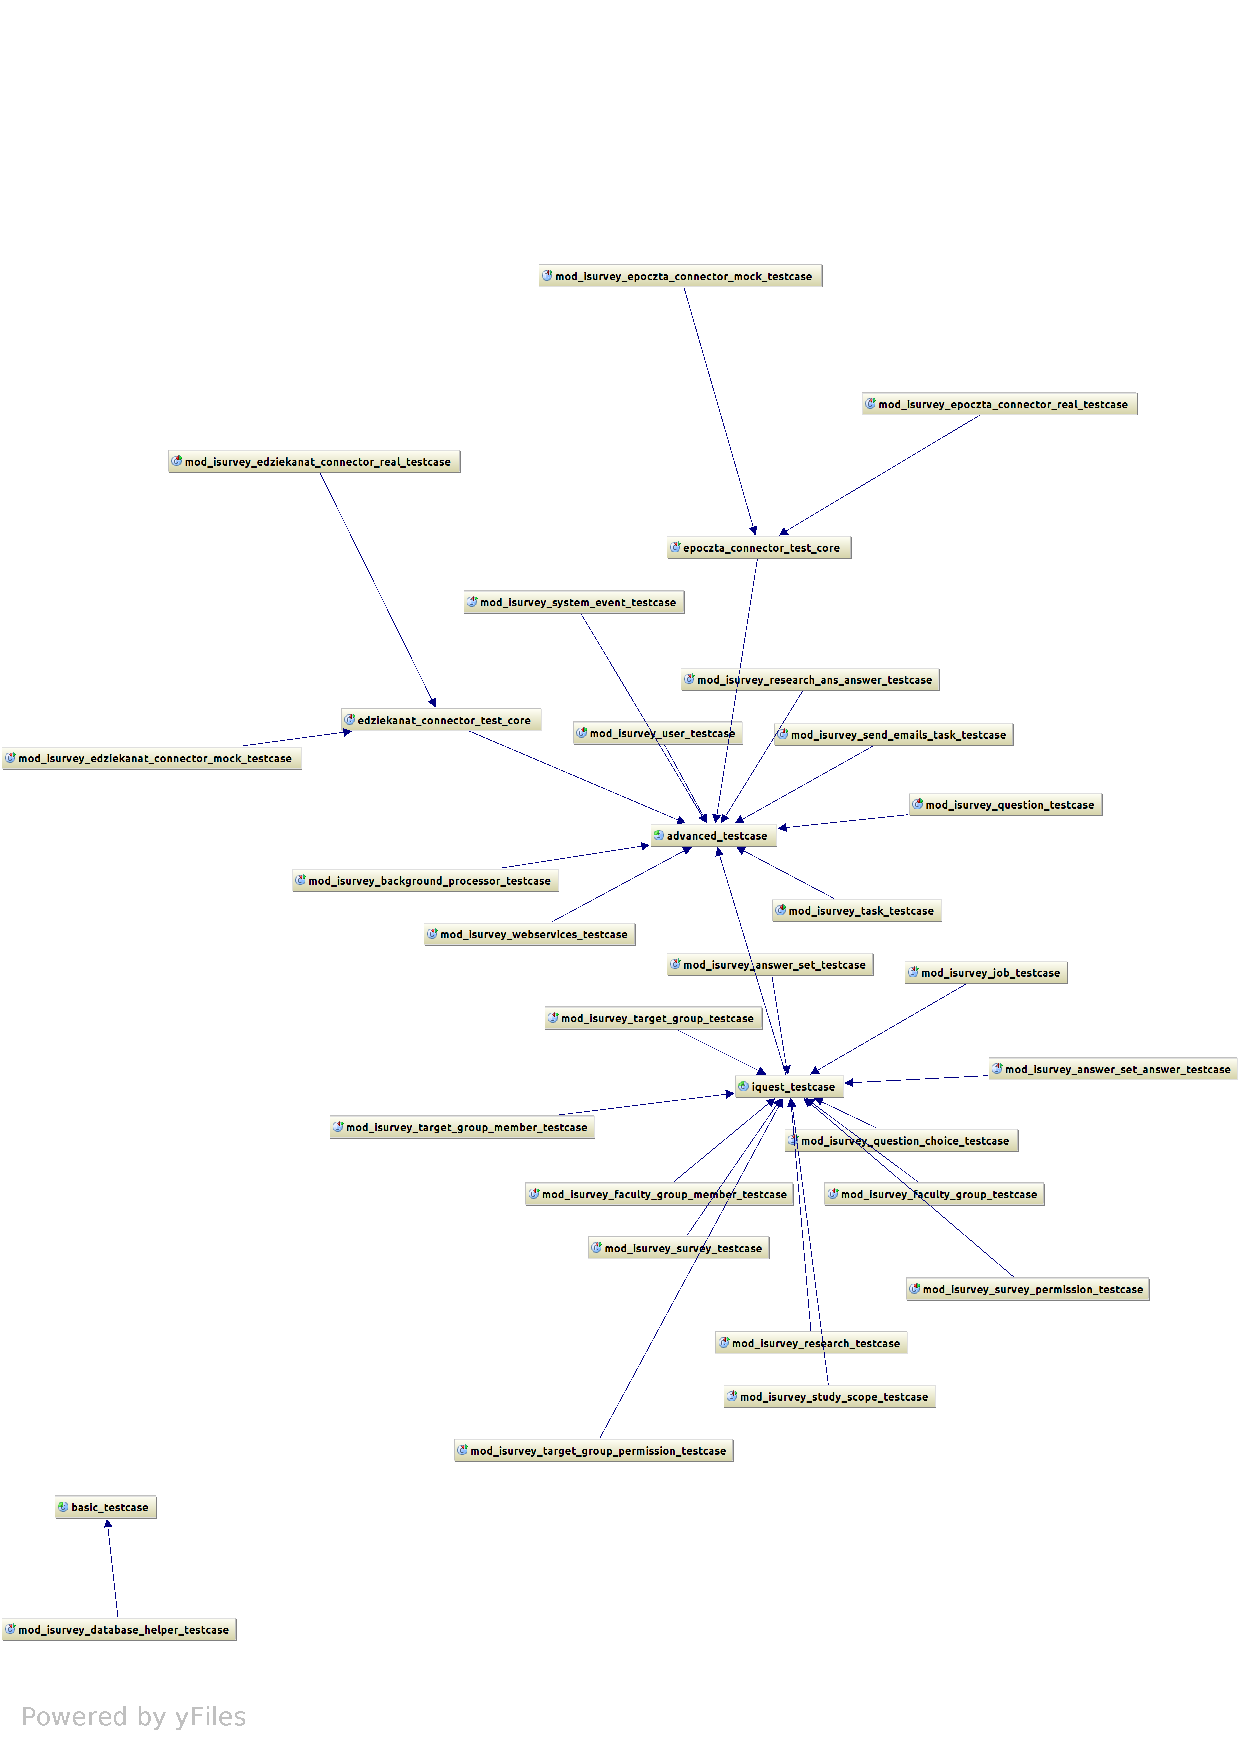
\includegraphics[width=0.9\textwidth]{figures/lw/tests.pdf} 
\end{center}
\caption{Struktura klas testujących}
\label{fig:tests}
\end{figure}

\subsection{Testy akceptacyjne}
\label{Chapter713}

Testy akceptacyjne rozpatrywane są na dwóch poziomach: automatycznym i manualnym. Różnica polega jedynie na tym, kto (lub co) wykonuje test - komputer z odpowiednim oprogramowaniem, czy człowiek.

\subsubsection{MAT}
\label{Chapter7131}
{\color{red}Testy akceptacyjne wymagają poprawienia -- dane od zespołu zarządzającego były nieaktualne!!!}
Poniżej przedstawiono Manualne Testy Akceptacyjne:

\matbegin{TC1}{Logowanie do systemu przez eKonto}
\matpres
\matpre{Użytkownik jest niezalogowany}
\matpre{Użytkownik posiada eKonto}
\matpre{Połączenie z Internetem}
\matsteps
\matstep{1}{Użytkownik wpisuje adres systemu}{Strona logowania do system iQuest}
\matstep{2}{Użytkownik naciska przycisk ,,Zaloguj przez eKonto''}{Strona logowania eLogin}
\matstep{3}{Użytkownik wpisuje dane logowania}{}
\matstep{4}{Użytkownik naciska przycisk ,,Zaloguj''}{Przekierowanie na stronę systemu iQuest, wyświetlenie strony głównej z zalogowanym użytkownikiem.}
\matremark{}

\matbegin{TC2}{Stworzenie Ankiety}
\matpres
\matpre{Zalogowany użytkownik z prawem do tworzenia ankiet}
\matsteps
\matstep{1}{Użytkownik wybiera przycisk ,,Stwórz ankietę''}{Strona umożliwiająca tworzenie ankiet}
\matstep{2}{Użytkownik podaje nazwę ankiety}{}
\matstep{3}{Użytkownik podaje wstęp  i podsumowanie ankiety}{}
\matstep{4}{Użytkownik dodaje pytanie jednokrotnego wyboru}{Pojawia się pole na wpisanie treści pytania}
\matstep{5}{Użytkownik wpisuje treść pytania}{}
\matstep{6}{Użytkownik naciska przycisk „Dodaj odpowiedź'' dwukrotnie}{Pojawiają się dwa pola do wpisania możliwych odpowiedzi}
\matstep{7}{Użytkownik podaje treści możliwych odpowiedzi}{}
\matstep{8}{Użytkownik dodaje stronę wciskając przycisk „Dodaj stronę''}{Wyświetla się nowa strona na dodawanie pytań}
\matstep{9}{Użytkownik dodaje pytanie otwarte}{Wyświetla się pole na wpisanie treści pytania}
\matstep{10}{Użytkownik wpisuje treść pytania}{}
\matstep{11}{Użytkownik wybiera przycisk „Zapisz zmiany''}{Komunikat o pomyślnym stworzeniu ankiety}
\matremark{}

\begin{table}[H]
\centering
\begin{tabular}{ | >{\bfseries}c | p{5cm} | } \hline
Krok & \textbf{Dane} \\ \hline
2 & ,,Ankieta testowa'' \\ \hline
3 & ,,Wstęp'' oraz ,,Podsumowanie'' \\ \hline
5 & ,,Pytania jednokrotnego wyboru działają?'' \\ \hline
7 & ,,tak'' oraz ,,nie'' \\ \hline
10 & ,,Pytania otwarte działają?'' \\ \hline
\end{tabular}
\caption{Poprawne dane dla scenariusza TC2}\label{tab:TC2-correct}
\end{table}

\matbegin{TC2.2}{Stworzenie Ankiety - brak pytań}
\matpres
\matpre{Zalogowany użytkownik z prawem do tworzenia ankiet}
\matsteps
\matstep{1}{Użytkownik wybiera przycisk „Stwórz ankietę''}{Strona umożliwiająca tworzenie ankiet}
\matstep{2}{Użytkownik podaje nazwę ankiety}{}
\matstep{3}{Użytkownik podaje wstęp  i podsumowanie ankiety}{}
\matstep{4}{Użytkownik wybiera przycisk „Zapisz zmiany''}{Komunikat o braku pytań w ankiecie}
\matremark{}

\matbegin{TC3}{Edycja ankiety}
\matpres
\matpre{Zalogowany użytkownik z prawem do tworzenia ankiet}
\matpre{Użytkownik posiada prawo do edycji ankiety ,,Ankiety testowej''}
\matsteps
\matstep{1}{Użytkownik wybiera przycisk „Katalog Ankiet''}{Strona z listą ankiet do których prawo ma użytkownik.}
\matstep{2}{Użytkownik wybiera przycisk „edytuj'' przy „Ankiecie Testowej''}{Strona umożliwiająca edycję „Ankiety Testowej''}
\matstep{3}{Użytkownik wciska przycisk „usuń'' przy pytaniu drugim}{Pytanie drugie znika}
\matstep{4}{Użytkownik naciska przycisk „Dodaj odpowiedź'' przy pytaniu pierwszym}{Pojawia się pole do wpisania możliwej odpowiedzi}
\matstep{5}{Użytkownik wpisuje możliwą odpowiedź}{}
\matstep{6}{Użytkownik wybiera przycisk „Zapisz zmiany''}{Strona wyświetla komunikat potwierdzający zapisanie zmian w ankiecie.}
\matremark{}

\begin{table}[H]
\centering
\begin{tabular}{ | >{\bfseries}c | p{5cm} | } \hline
Krok & \textbf{Dane} \\ \hline
5 & ,,nie wiem'' \\ \hline
\end{tabular}
\caption{Poprawne dane dla scenariusza TC3}\label{tab:TC3-correct}
\end{table}

\matbegin{TC3}{Edycja ankiety - usunięcie wszystkich pytań}
\matpres
\matpre{Zalogowany użytkownik z prawem do tworzenia ankiet}
\matpre{Użytkownik posiada prawo do edycji ankiety ,,Ankiety testowej''}
\matsteps
\matstep{1}{Użytkownik wybiera przycisk „Katalog Ankiet''}{Strona z listą ankiet do których prawo ma użytkownik.}
\matstep{2}{Użytkownik wybiera przycisk „edytuj'' przy „Ankiecie Testowej''}{Strona umożliwiająca edycję „Ankiety Testowej''}
\matstep{3}{Użytkownik wciska przycisk „usuń'' przy każdym z pytań}{Pytania znikają}
\matstep{4}{Użytkownik wybiera przycisk „Zapisz zmiany''}{Strona wyświetla komunikat, że ankieta nie posiada pytań i prosi o ich dodanie.}
\matremark{}

\matbegin{TC4}{Wybranie grupy docelowej}
\matpres
\matpre{Zalogowany użytkownik z prawami do tworzenia ankiet}
\matpre{Użytkownik posiada prawa do ankiety „Ankieta Testowa''}
\matpre{Użytkownik posiada prawo do ankietowania grupy docelowej „test''}
\matsteps
\matstep{1}{Użytkownik wybiera przycisk ,,Włącz tryb edycji''}{Interfejs edycji Moodle}
\matstep{2}{Użytkownik wybiera przycisk „edytuj'' przy „Ankiecie Testowej''}{Strona umożliwiająca edycję „Ankiety Testowej''}
\matstep{3}{Użytkownik wybiera grupę docelową „test''}{}
\matstep{4}{Użytkownik wybiera przycisk „Zapisz zmiany''}{Strona wyświetla komunikat, że ankieta została zaktualizowana pomyślnie.}
\matstep{5}{Respondent otrzymuje email z powiadomieniem o ankiecie}{}
\matremark{}

\matbegin{TC5}{Udzielanie odpowiedzi}
\matpres
\matpre{Zalogowany użytkownik}
\matpre{Użytkownik znajduje się w grupie docelowej ankiety ,,testowa''}
\matpre{Użytkownik nie odpowiadał udzielał odpowiedzi na ankietę ,,testowa''}
\matsteps
\matstep{1}{System prezentuje ankiety na które użytkownik jeszcze nie odpowiedział}{}
\matstep{2}{Użytkownik wybiera ankietę ,,testowa''}{System prezentuje ankietę}
\matstep{3}{Użytkownik zaznacza odpowiedź na pytanie 1 jako ,,tak''}{}
\matstep{4}{Użytkownik podaje odpowiedź na pytanie drugie jako ,,tak''}{}
\matstep{5}{Użytkownik potwierdza wypełnienie ankiety przyciskiem ,,Wyślij''}{System prezentuje ankiety na które użytkownik jeszcze nie odpowiedział oraz komunikat o pomyślnym przesłaniu odpowiedzi}
\matstep{6}{Respondent otrzymuje email z powiadomieniem o ankiecie}{}
\matremark{}

\matbegin{TC6}{Sprawdzenie wyników}
\matpres
\matpre{Zalogowany użytkownik z prawem do oglądania wyników ankiety ,,Testowa''}
\matsteps
\matstep{1}{Użytkownik wybiera badanie, którego podstawowe wyniki chce sprawdzić}{System prezentuje podsumowanie ankiety}
\matremark{Dotyczy podstawowych wyników. Wyniki zaawansowane obsługuje zewnętrzny serwer BI}

\matbegin{TC7}{Dodawanie grupy docelowej}
\matpres
\matpre{Zalogowany administrator z prawami do tworzenia grup docelowych}
\matpre{Brak w systemie grupy docelowej ,,Grupa 1''}
\matsteps
\matstep{1}{Administrator wybiera przycisk ,,Zarządzaj grupami docelowymi''}{System prezentuje dostępne grupy docelowe w systemie}
\matstep{2}{Administrator wybiera przycisk ,,dodaj''}{System prezentuje interfejs dodawania grupy docelowej}
\matstep{3}{Administrator podaję nazwę nowej grupy „Grupa 1” i wskazuje jej członków}{}
\matstep{4}{Administrator wybiera grupę nadrzędną dla nowej grupy docelowej}{System automatycznie zapisują zmiany}
\matremark{Test przygotowany na podstawie makiety systemu iQuest}

\matbegin{TC8}{Edycja grupy docelowej}
\matpres
\matpre{Zalogowany administrator z prawami do tworzenia grup docelowych}
\matpre{Grupa docelowa ,,Grupa 1'' istnieje w systemie}
\matsteps
\matstep{1}{Administrator wybiera przycisk ,,Zarządzaj grupami docelowymi''}{System prezentuje dostępne grupy docelowe w systemie}
\matstep{2}{Administrator wybiera przycisk ,,zmień nazwę''}{System prezentuje interfejs zmiany nazwy grupy docelowej}
\matstep{3}{Administrator pozostawia nazwę niezmienioną i zatwierdza zmiany}{System prezentuje dostępne grupy docelowe w systemie}
\matstep{4}{Administrator wybiera grupę nadrzędną dla grupy docelowej i dodaje nowego członka do grupy}{System automatycznie zapisują zmiany}
\matremark{Test przygotowany na podstawie makiety systemu iQuest}

\matbegin{TC9}{Edycja grupy docelowej}
\matpres
\matpre{Użytkownik jest niezalogowany}
\matpre{Istnieje konto użytkownika w systemie}
\matsteps
\matstep{1}{Użytkownik wpisuje adres systemu}{Strona główna moodla z kursem iQuest}
\matstep{2}{Użytkownik naciska przycisk ,,Zaloguj się''}{Strona logowania}
\matstep{3}{Użytkownik wpisuje dane logowania}{}
\matstep{4}{Użytkownik naciska przycisk ,,Zaloguj się''}{Przekierowanie na główną stronę moodla z kursem iQuest. Wyświetla się napis: ,,Jesteś zalogowany(a) jako...''}
\matremark{}

{\color{red}Niedodane jeszcze TC: Logowanie bez eKonta, }

Dodatkowo, poniżej znajduje się wykaz mapujący przypadki testowe do przypadków użycia:
\begin{itemize}
\item{TC1.X – UC09 Logowanie do systemu.}
\item{TC2.X – UC01 Stworzenie ankiety}
\item{TC3.X – UC02 Edycja ankiety}
\item{TC4.X – UC03 UC04 Wybranie grupy docelowej, uruchomienie ankiety}
\item{TC5.X – UC05 Udzielenie odpowiedzi}
\item{TC6.X – UC06 Sprawdzenie wyników}
\item{TC7.X – UC07 Tworzenie grupy docelowej}
\item{TC8.X – UC08 Edycja grupy docelowej}
\item{TC9.X – UC09 Logowanie do systemu}
\end{itemize}

\subsubsection{AAT}
\label{Chapter7131}

Automatyczne testy akceptacyjne realizowano w zgodzie z testami manualnymi i operując na tych samych wytycznych. Nagrywanie testów odbywało się za pomocą oprogramowania Selenium IDE, udostępnianego w formie rozszerzenia dla przeglądarki Mozilla Firefox. Pierwotnie, testy były konwertowane do języka Java, celem uruchamiania ich z poziomu języka Java, oferującego sporą swobodę przy projektowaniu warunków początkowych i końcowych dla testów. Problemy, jakie wynikały z takiego działania, opisane zostały w rozdziale \ref{Chapter6}. Na ich podstawie zdecydowano o pozostaniu w obrębie Selenium IDE, które samo w sobie również umożliwia automatyzację w wysokim stopniu. Aby dodatkowo ułatwić zadanie, przygotowany został skrypt ustawiający bazę danych w stan początkowy dla realizacji testów.

\subsection{Inne metody zapewniania jakości}
\label{Chapter714}

Celem zapewnienia jak najwyższej jakości oprogramowania, było ono testowane -- w kontrolowanych warunkach -- na różnorakich maszynach. Co prawda, lokalne serwery developerskie pracowały w oparciu o system Ubuntu 12.04 LTS, z serwerem Apache i systemem zarządzania bazą danych PostgreSQL, jednak maszyny klienckie były już znacznie bardziej różnorodne.

System przetestowano na zbiorze komputerów stacjonarnych klasy PC oraz równoważnych laptopów, z użyciem systemów Windows i Linux. Realizowano je także na laptopach i netbookach klasy PC oraz Macintosh, również pod kontrolą systemów Windows i Linux, oraz - w przypadku tej ostatniej klasy - MacOS. Ponadto, przetestowano trzy główne platformy mobilne (Android, iOS, WP7.x) poprzez dostęp do systemu z poziomu telefonów komórkowych.

Wspomniane wyżej maszyny pracowały pod kontrolą następujących systemów operacyjnych:
\begin{itemize}
\item{Windows XP Professional SP3 32-bit + Internet Explorer 7}
\item{Windows Vista Business SP2 32-bit + Internet Explorer 8}
\item{Windows 7 Professional SP1 64-bit + Mozilla Firefox + Google Chrome}
\item{Windows 8 Professional 64-bit + Internet Explorer 10 + Google Chrome}
\item{Ubuntu 12.04 64-bit + Mozilla Firefox + Google Chrome}
\item{Mac OS X + Apple Safari}
\item{Google Android 2.2, 2.3, 4.0, 4.1}
\item{iOS (iPhone 4S)}
\item{Windows Phone 7.5 (Nokia Lumia 710)}
\end{itemize}

Na podstawie powyższych testów, utworzono dwa raporty: ,,wygląd i działanie systemu iQuest na platformach mobilnych'' oraz ,,wygląd i działanie systemu iQuest w różnych konfiguracjach system-przeglądarka'', udostępnione w ramach systemu zarządzania projektem\cite{Redmine:ProjDocs}. Wynika z nich, że system iQuest posiada bardzo wysoki współczynnik przenośności.